\documentclass[xcolor={usenames,svgnames}]{beamer}

\usepackage[francais]{babel}
\usepackage{rtxslides}
\usepackage{listings}
\usepackage{tikz}
\usetikzlibrary{shapes,fit}

\newcommand{\bgcolor}{black}
\newcommand{\fgcolor}{white}

\lstdefinelanguage{rathaxes}%
{
	morekeywords={
        interface, extend,                      % interfaces : decl
        device, configuration, driver,          % devices
        with, values,                           % backend+interface
        builtin, provided, required, optional,  % interfaces: implem
        type, sequence, variable,               % general: element type
        pointcut, chunk,                        % for aspectual concepts
        template                                % backend
    },%
	morecomment=[l][\color{Gainsboro}]{//},%
 	morecomment=[l][\color{Gainsboro}]{\#},%
	morecomment=[s][\color{Gainsboro}]{/*}{*/},%
	morestring=[b][\color{Gold}]",%
	morestring=[b][\color{Gold}]',%
	keywordstyle={\color{Tomato}}%
}[keywords,comments,strings]

\lstset{
    language=rathaxes,
    tabsize=4,
    captionpos=b,
    emptylines=0,
    breaklines=false,
    breakatwhitespace=false,        % sets if automatic breaks should only happen at whitespace
    extendedchars=false,
    showstringspaces=false,
    showspaces=false,
    numbersep=1ex,
    showtabs=false,
    basicstyle=\color{white}\scriptsize\ttfamily,
    numberstyle=\color{Gainsboro}\scriptsize\ttfamily,
    stepnumber=1,                   % the step between two line-numbers. If it's 1, each line
    keywordstyle=\color{Tomato},
    commentstyle=\color{Gainsboro},
    stringstyle=\color{white},
    backgroundcolor=\color{black},
    escapeinside={\%*}{*)},         % if you want to add a comment within your code
    morekeywords={*,...}            % if you want to add more keywords to the set
}

\title{\rtx, a DSL for device drivers}
\date[Soutenance Finale Ept5]{Soutenance Finale Ept5 \\ \vspace{10pt} 
\includegraphics[height=12mm]{logo_eip}}
\author[\rtx\ 2012 -- 11 février 2012]{\rtx\ 2012 -- 11 février 2012 \vspace{-20pt}}

\definecolor{lightred}{RGB}{147,36,33}
\newcommand{\cemph}[1]{{\itshape\LARGE{\textcolor{rathaxesred}{#1}}}}

\setbeamertemplate{navigation symbols}{}

\tikzset{textbox/.style={draw, ultra thick, color=rathaxesred, rectangle, text=\fgcolor, rounded corners=3pt}}
\tikzset{warrow/.style={->, >=stealth, color=\fgcolor, ultra thick}}
\tikzset{graybox/.style={draw,rectangle,rounded corners=3pt,very thick,densely dashed,color=gray!75,text=\fgcolor}}
\tikzset{redcontainer/.style={draw,rectangle,rounded corners=5pt,ultra thick,color=rathaxesred,text=\fgcoor,minimum height=3.5cm,minimum width=2.5cm}}
\tikzset{redbox/.style={draw,rectangle,rounded corners=5pt,ultra thick,color=rathaxesred,text=\fgcolor}}

\begin{document}

\begin{frame}
\titlepage
\end{frame}

\begin{frame}{EIP $\rightarrow$ Epitech Innovative Project}
\Large{
\begin{itemize}
\item Covers the 2 last years of studies;
\item At least 5 students;
\item Driven by the EIP Lab.
\end{itemize}
}
\end{frame}

\begin{frame}{Rathaxes goal}
\Large{
\textrm{\itshape{``\rtx\ is a \textcolor{rathaxesred}{dedicated language} to
\textcolor{rathaxesred}{write peripherals drivers}. \rtx\ compiles to kernel
modules written in C for any defined operating system.''}}
\vspace{2em}
\begin{itemize}
\item LSE research project;
\item Solve driver development problematics.
\end{itemize}
}
\end{frame}

\begin{frame}{People concerned by Rathaxes}
\Large{
\begin{itemize}
\item Operating System researchers/developers;
\item Small companies with homemade hardware.
\end{itemize}
}
\end{frame}

\begin{frame}[fragile]{Our EIP group}
\begin{center}
\begin{tikzpicture}[overlay]
\node[redbox] (ZOBI) at (0, 2) {\begin{minipage}{46mm}\begin{center}Thomas Luquet \\ \small{\emph{Communication Leader}}\end{center}\end{minipage}};

\node[redbox] (ZO) at (-3, 0) {\begin{minipage}{46mm}\begin{center}Zoltan Konarzweski \\ \small{\emph{Language \& Compiler}}\end{center}\end{minipage}};
\node[redbox] (JOA) at (3, 0) {\begin{minipage}{46mm}\begin{center}David Pineau \\ \small{\emph{Language \& Compiler}}\end{center}\end{minipage}};

\node[redbox] (KAL) at (-3, -2) {\begin{minipage}{46mm}\begin{center}Louis Opter \\ \small{\emph{Unix drivers \& Maintainer}}\end{center}\end{minipage}};
\node[redbox] (DAEDRIC) at (3, -2) {\begin{minipage}{46mm}\begin{center}Thomas Sanchez \\ \small{\emph{Unix \& Windows drivers}}\end{center}\end{minipage}};
\end{tikzpicture}
\end{center}
\end{frame}

\begin{frame}{Origine du projet}
\Large{
\begin{itemize}
\item \rtx\ 2009 ;
\item Améliorer le développement de pilotes ;
\item Thèse de L. Réveillère \emph{«~Devil~»} (2002).
\end{itemize}
}
\end{frame}

\begin{frame}{Problématiques}
\Large{
\begin{itemize}
\item Compétences multiples ;
\item Code critique ; % non seulement en terme de fiabilité mais aussi en terme de debug
\item « Réutilisabilité » du code. % à la fois en terme de portabilité mais aussi en interne il y a beaucoup de répétitions.
\end{itemize}
}
\end{frame}

\begin{frame}{\rtx\ 2012}
\Large{
\begin{itemize}
\item Reprise du concept de DSL \& Compilateur ;
\item Reprise d'une partie du Front-end (\texttt{.rtx}) ;
\item Élargissement du langage ;
\item Nouveau modèle de génération.
\end{itemize}
\uncover<2->{\vspace{1em}{\LARGE \emph{Permettre à différentes personnes d'écrire différentes parties du pilote.}}}
}
\end{frame}

\begin{frame}[fragile]{Fonctionnement}
\begin{tikzpicture}[overlay]
\node (RTX) at (1,0) {
\includegraphics[height=1.5cm]{icons/rtx}};
\end{tikzpicture}
\end{frame}

\begin{frame}[fragile]{Fonctionnement}
\begin{tikzpicture}[overlay]
\node (RTX) at (1,0) {
\includegraphics[height=1.5cm]{icons/rtx}};

\node[redbox] (COMPILER) at (5.5,0) {\LARGE{Rathaxes}};

\draw[warrow] (RTX)--(COMPILER);
\end{tikzpicture}
\end{frame}

\begin{frame}[fragile]{Fonctionnement}
\begin{tikzpicture}[overlay]
\node (RTX) at (1,0) {
\includegraphics[height=1.5cm]{icons/rtx}};

\node[redbox] (COMPILER) at (5.5,0) {\LARGE{Rathaxes}};

\draw[warrow] (RTX)--(COMPILER);

\node (WDRV) at (10, 2.5) {
\includegraphics[height=2cm]{medias/driverbox}};

\node (LDRV) at (10, 0) {
\includegraphics[height=2cm]{medias/driverbox}};

\node (OTHER) at (10, -2.5) {
\includegraphics[height=2cm]{medias/driverbox}};

\draw (LDRV.north east) node[below left] {
\includegraphics[height=1.5cm]{medias/tux}};

\draw (WDRV.north east) node[below left] {
\includegraphics[height=1.3cm]{medias/windows_no_text}};

\draw (OTHER.north east) node[below left] {\Large{\ldots}};

\draw[warrow] (COMPILER.east)--(WDRV.south west);
\draw[warrow] (COMPILER.east)--(LDRV);
\draw[warrow] (COMPILER.east)--(OTHER.north west);
\end{tikzpicture}
\end{frame}

\begin{frame}
\begin{center}
\emph{\Huge{Démonstration}}
\end{center}
\end{frame}

\begin{frame}{Communication}
\begin{center}
\begin{tikzpicture}
\node (RMLL) at (0, 0) {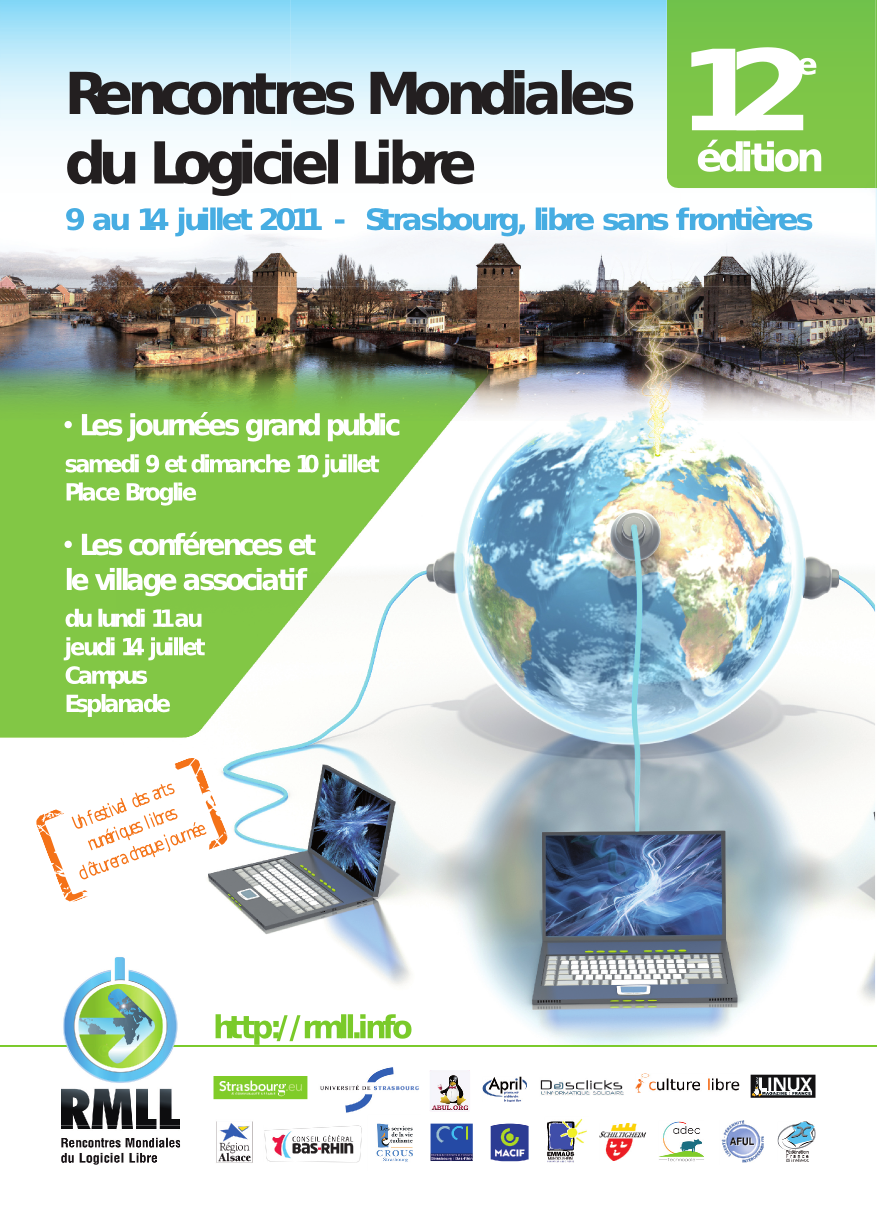
\includegraphics[height=6cm]{rmll_2011}};

\draw (RMLL.east) node[right] {\begin{minipage}{45mm}\begin{itemize}
\item \Large{RMLL 2011} ;
\item \Large{Youtube} ;
\end{itemize}\end{minipage}};
\end{tikzpicture}
\end{center}
\end{frame}

\begin{frame}{Communication}
\begin{center}
\begin{tikzpicture}
\node (RMLL) at (0, 0) {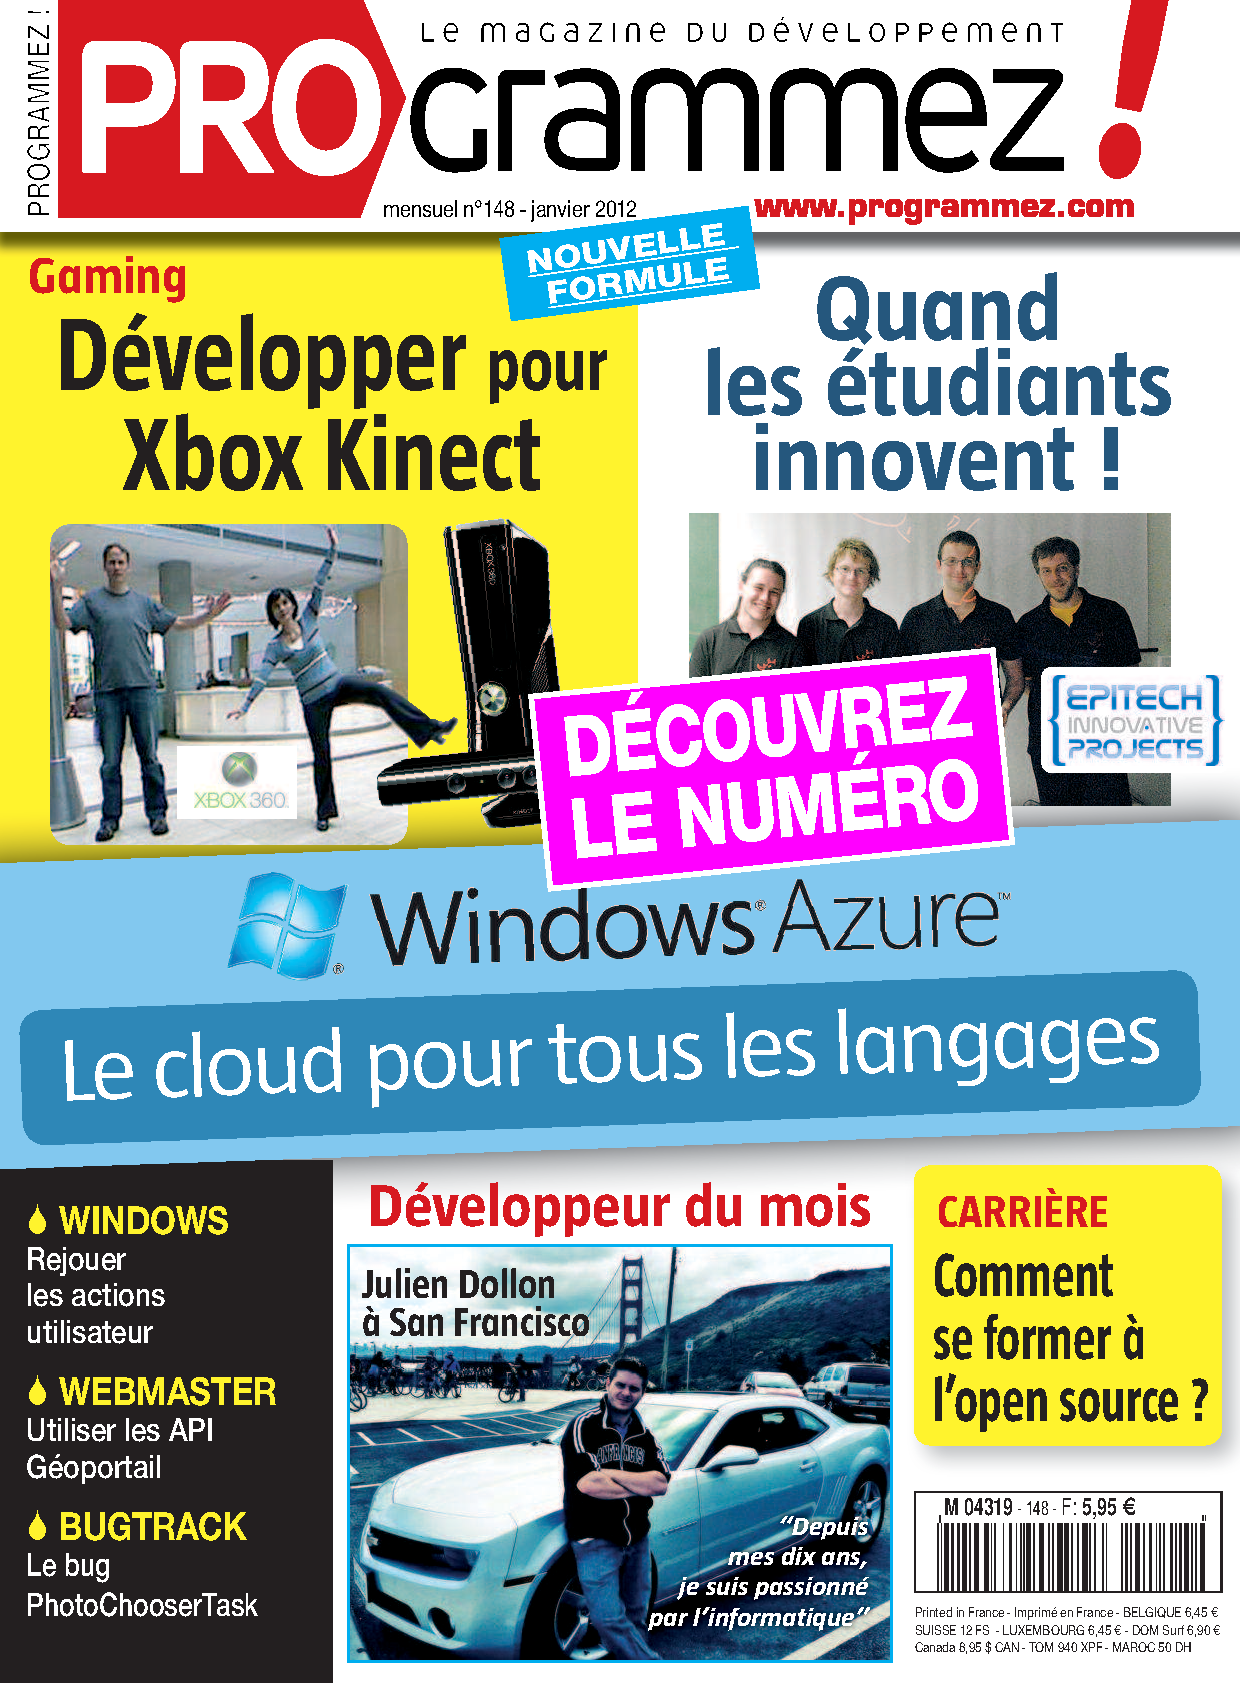
\includegraphics[height=6cm]{programmez}};

\draw (RMLL.east) node[right] {\begin{minipage}{45mm}\begin{itemize}
\item \Large{Couverture de \itshape{Programmez!}}
\end{itemize}\end{minipage}};
\end{tikzpicture}
\end{center}
\end{frame}

\begin{frame}{Communication}
\begin{center}
\begin{tikzpicture}
\node (FOSDEM) at (0, 0) {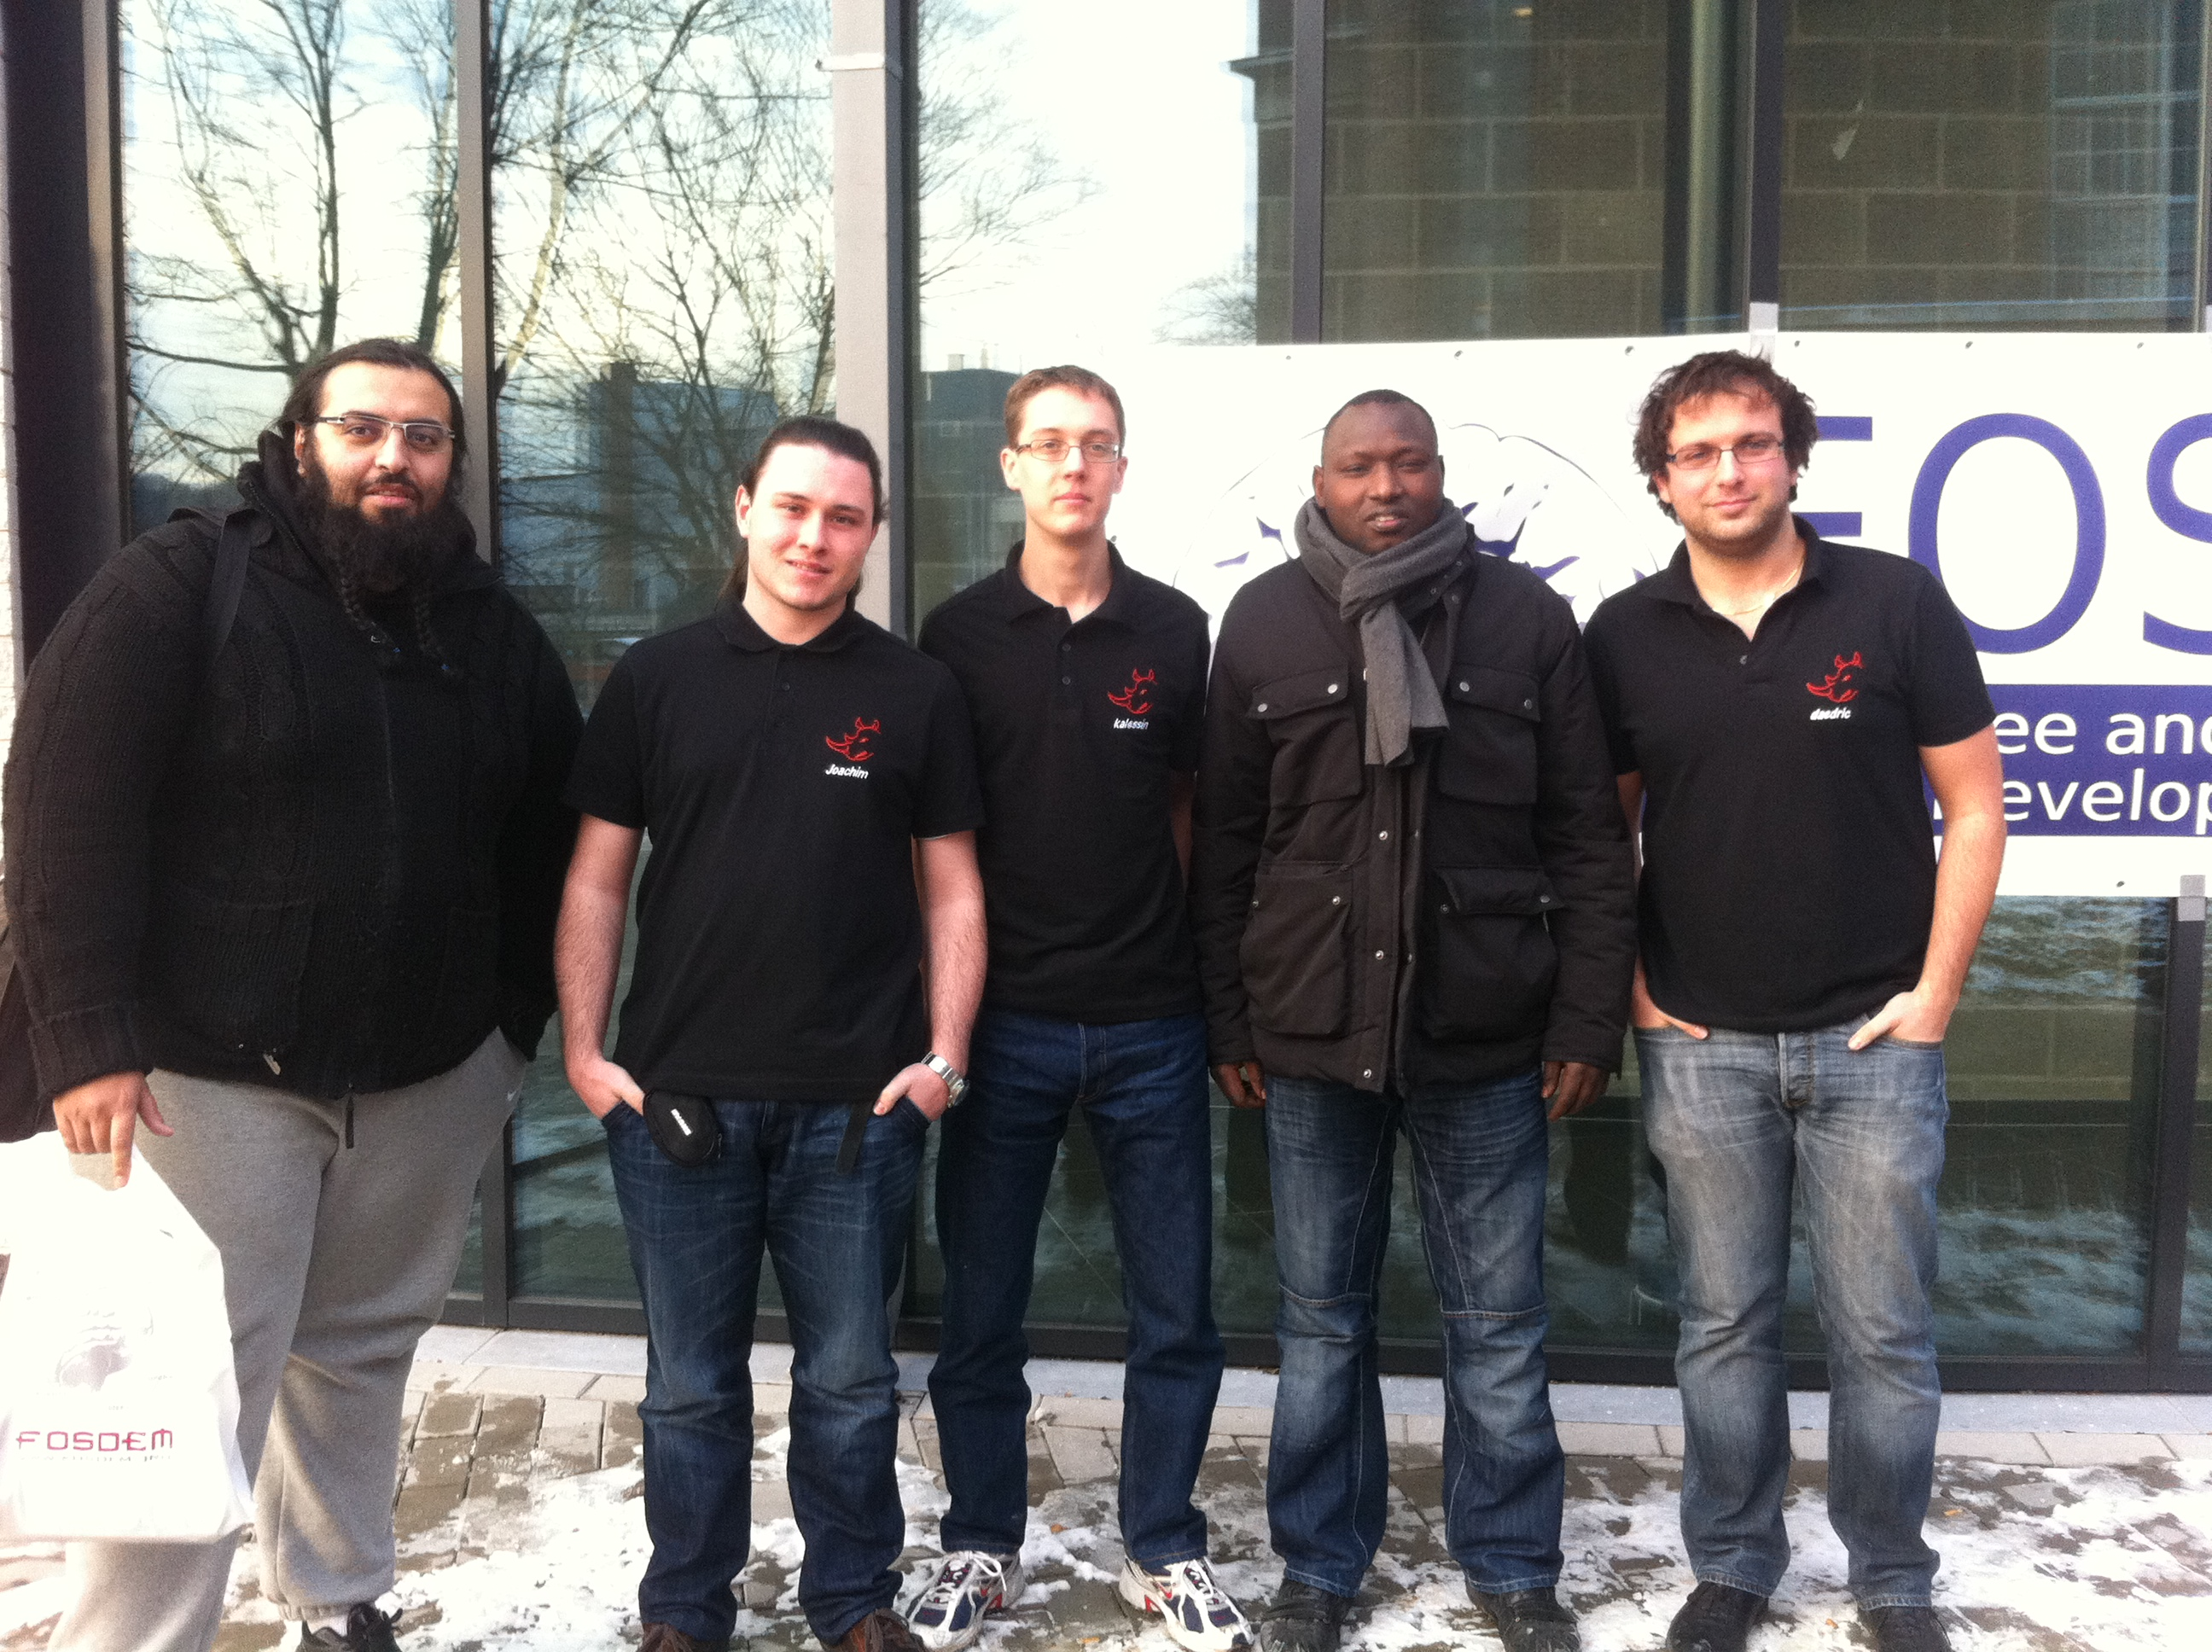
\includegraphics[height=6cm]{fosdem_2012}};

\draw (FOSDEM.south) node[below] {\Large{\emph{Fosdem 2012}}};
\end{tikzpicture}
\end{center}
\end{frame}

\begin{frame}[fragile]{Conduite de projet}
\begin{center}
\begin{tikzpicture}[overlay]
\node (Ubuntu) at (-3.60, 1.5) {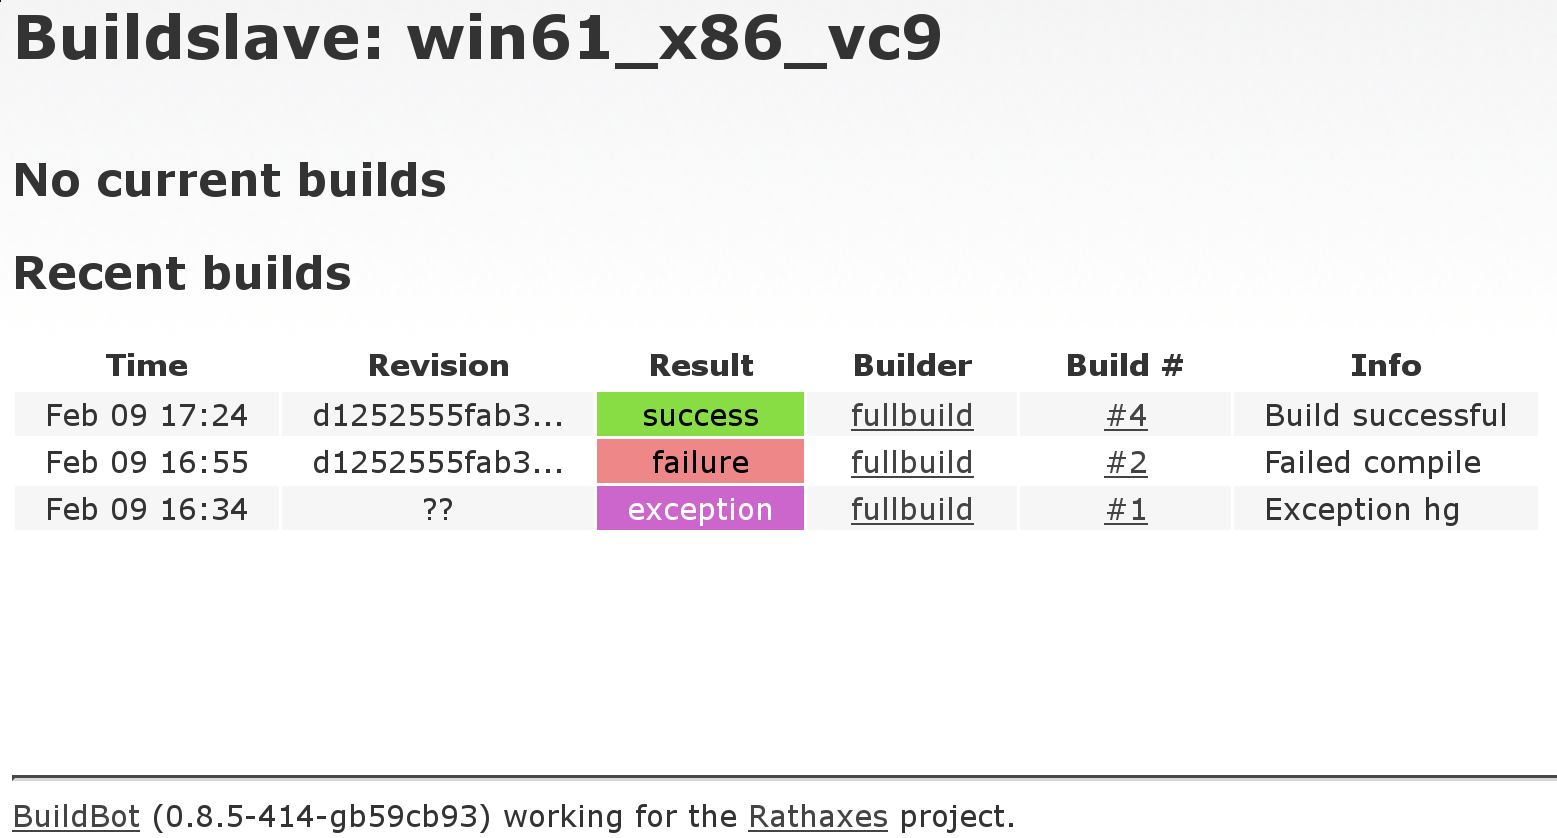
\includegraphics[scale=0.08]{medias/buildbot_windows}};
\node (Windows) at (-3.10, 0.25) {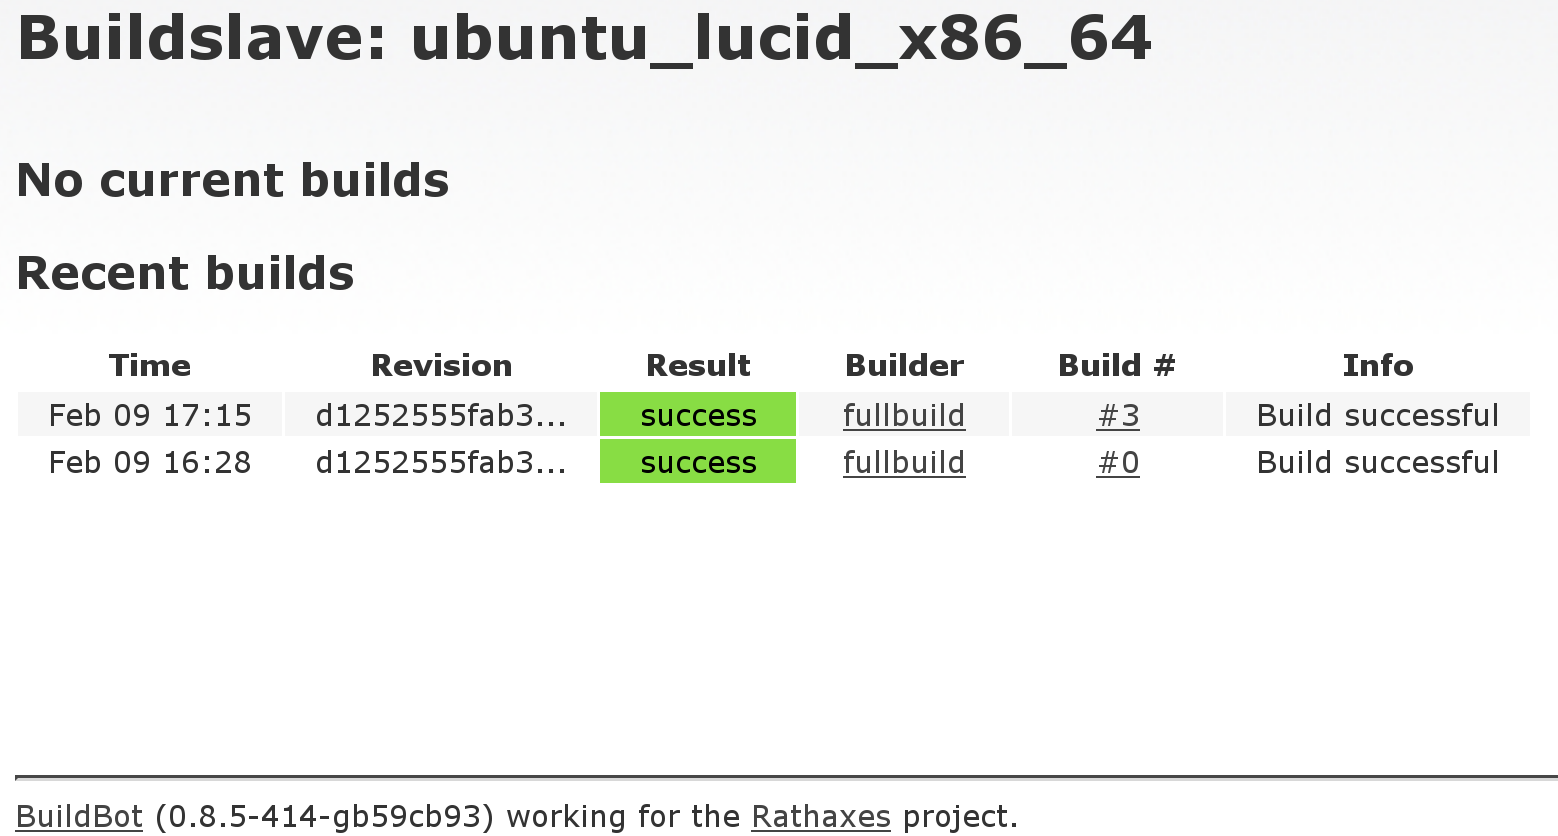
\includegraphics[scale=0.08]{medias/buildbot_ubuntu}};
\node (Gcode) at (-4.10, -2.50) {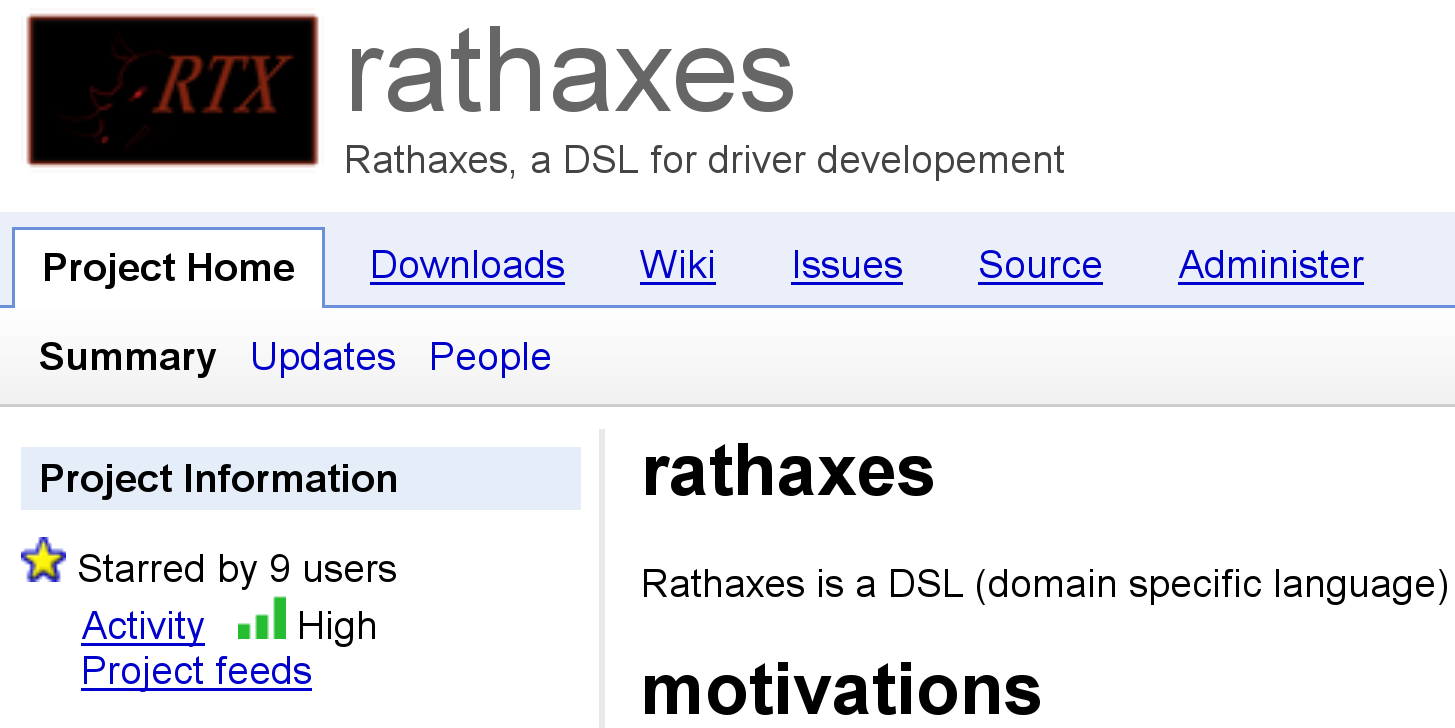
\includegraphics[scale=0.08]{medias/gcode}};
\draw (-1.10, 0) node[right] {\begin{minipage}{110mm}\begin{itemize}
\item \Large{Intégration Continue} ;
\item \Large{Google Code \& Mercurial} ;
\item \Large{IRC \& Skype}.
\end{itemize}\end{minipage}};
\end{tikzpicture}
\end{center}
\end{frame}

\begin{frame}{Conclusion}
\large{
\begin{itemize}
\item Passage en Open Source ;
\item Nouvelle version du langage et du compilateur ;
\item Génération de modules sous Linux et Windows ;
\item Pilote Linux PCI/Ethernet pour une carte Intel ;
\item \LARGE{\emph{Poursuite du projet.}}
\end{itemize}
}
\end{frame}

\begin{frame}{Merci}
\begin{center}
\Huge{\emph{Questions ?}}
\end{center}

\vspace{2em}
\begin{itemize}
\item \Large{\texttt{http://www.rathaxes.org/}}
\end{itemize}
\end{frame}

\setbeamertemplate{footline}{}

\begin{frame}[fragile]
\begin{center}
\begin{tikzpicture}[overlay]
\node (RTX) at (-1,0.5) {
\includegraphics[height=60mm]{logo_latex}};

\draw (0, -3.3) node {{\Huge\itshape{\textcolor{rathaxesred}{\rtx}}}};

\draw (5.3, -4.6) node {
\includegraphics[height=7mm]{logo_eip}};

\draw (3.5, -4.6) node {
\includegraphics[height=7mm]{logo_epitech}};
\end{tikzpicture}
\end{center}
\end{frame}

\end{document}
